%%%% This CV has been greatly influence by
%%%% the extended fancy cv from Carmine Benedetto.
%%%% I thank him for the excellent work. Unfortunately 
%%%% it wouldn't compile on my machine. So I worked it out myself.

\documentclass{article} 
\usepackage[ngerman]{babel}% deutsche Trennregeln
\usepackage{microtype}% verbesserter Randausgleich
\usepackage[utf8]{inputenc}
\usepackage{graphicx}
\usepackage{color}
\usepackage{xcolor}
\usepackage[obeyspaces]{url} 
\usepackage[left=0.5cm,top=0cm,right=0.5cm,bottom=0.5cm,nohead,nofoot]{geometry}

\usepackage{fontawesome}
\usepackage{svg}

\makeatletter
\setlength{\@fptop}{40pt}
\makeatother



\usepackage{pdfcomment}
%% Fix incorrect display of tooltips (http://tex.stackexchange.com/a/74340/3323)
\makeatletter
\renewcommand{\pc@annot@tooltip}%
{%
  /TU (\pc@pdfenc@contents)\space%
  /T (tooltip \thezref@unique)\space%
  /C [0 0 0]\space%
  /FT/Btn\space%
  /Ff 65536\space%
  /H/N\space%
}%

\newcommand{\spacingWork}{0.25cm}
\newcommand{\minipageSmall}{0.13}
\newcommand{\minipageBig}{0.84}

\newcommand{\minipageSmallEd}{0.13}
\newcommand{\minipageBigEd}{0.84}
  
\definecolor{white}{RGB}{255,255,255}
\definecolor{anti-flashwhite}{rgb}{0.95, 0.95, 0.96}

\definecolor{darkgray}{HTML}{333333}
\definecolor{gray}{HTML}{4D4D4D}
\definecolor{lightgray}{HTML}{999999}

\definecolor{green}{HTML}{C2E15F}
\definecolor{orange}{HTML}{FDA333}
\definecolor{purple}{HTML}{D3A4F9}
\definecolor{red}{HTML}{FB4485}
\definecolor{blue}{HTML}{6CE0F1}
\definecolor{pblue}{HTML}{0395DE}

\usepackage{tikz}
\newcommand*{\ClipSep}{0.1cm}%


\usetikzlibrary{mindmap,shadows,positioning,backgrounds}

\renewcommand{\thempfootnote}{\arabic{mpfootnote}}

\usepackage{hyperref}
\hypersetup{
    pdftitle={},
    pdfauthor={},
    pdfsubject={},
    pdfkeywords={},
    colorlinks=false,       % no lik border color
   allbordercolors=white    % white border color for all
}

\pagestyle{empty}


%%%%%%%%%%%%%%%%%%%%%%%%%%%%%%%%%%%%%%%%%%%%%%%%%%%%%%%%%%%%%%%%%%%%%%%%%%%%%%%%%%%%%%%%%%%%%%%
\begin{document}
\noindent
\begin{minipage}[t]{0.25\textwidth}
	\vspace{0pt}
	\centering
%	\begin{tikzpicture}
%		\node [inner sep=0pt] at (0,0) {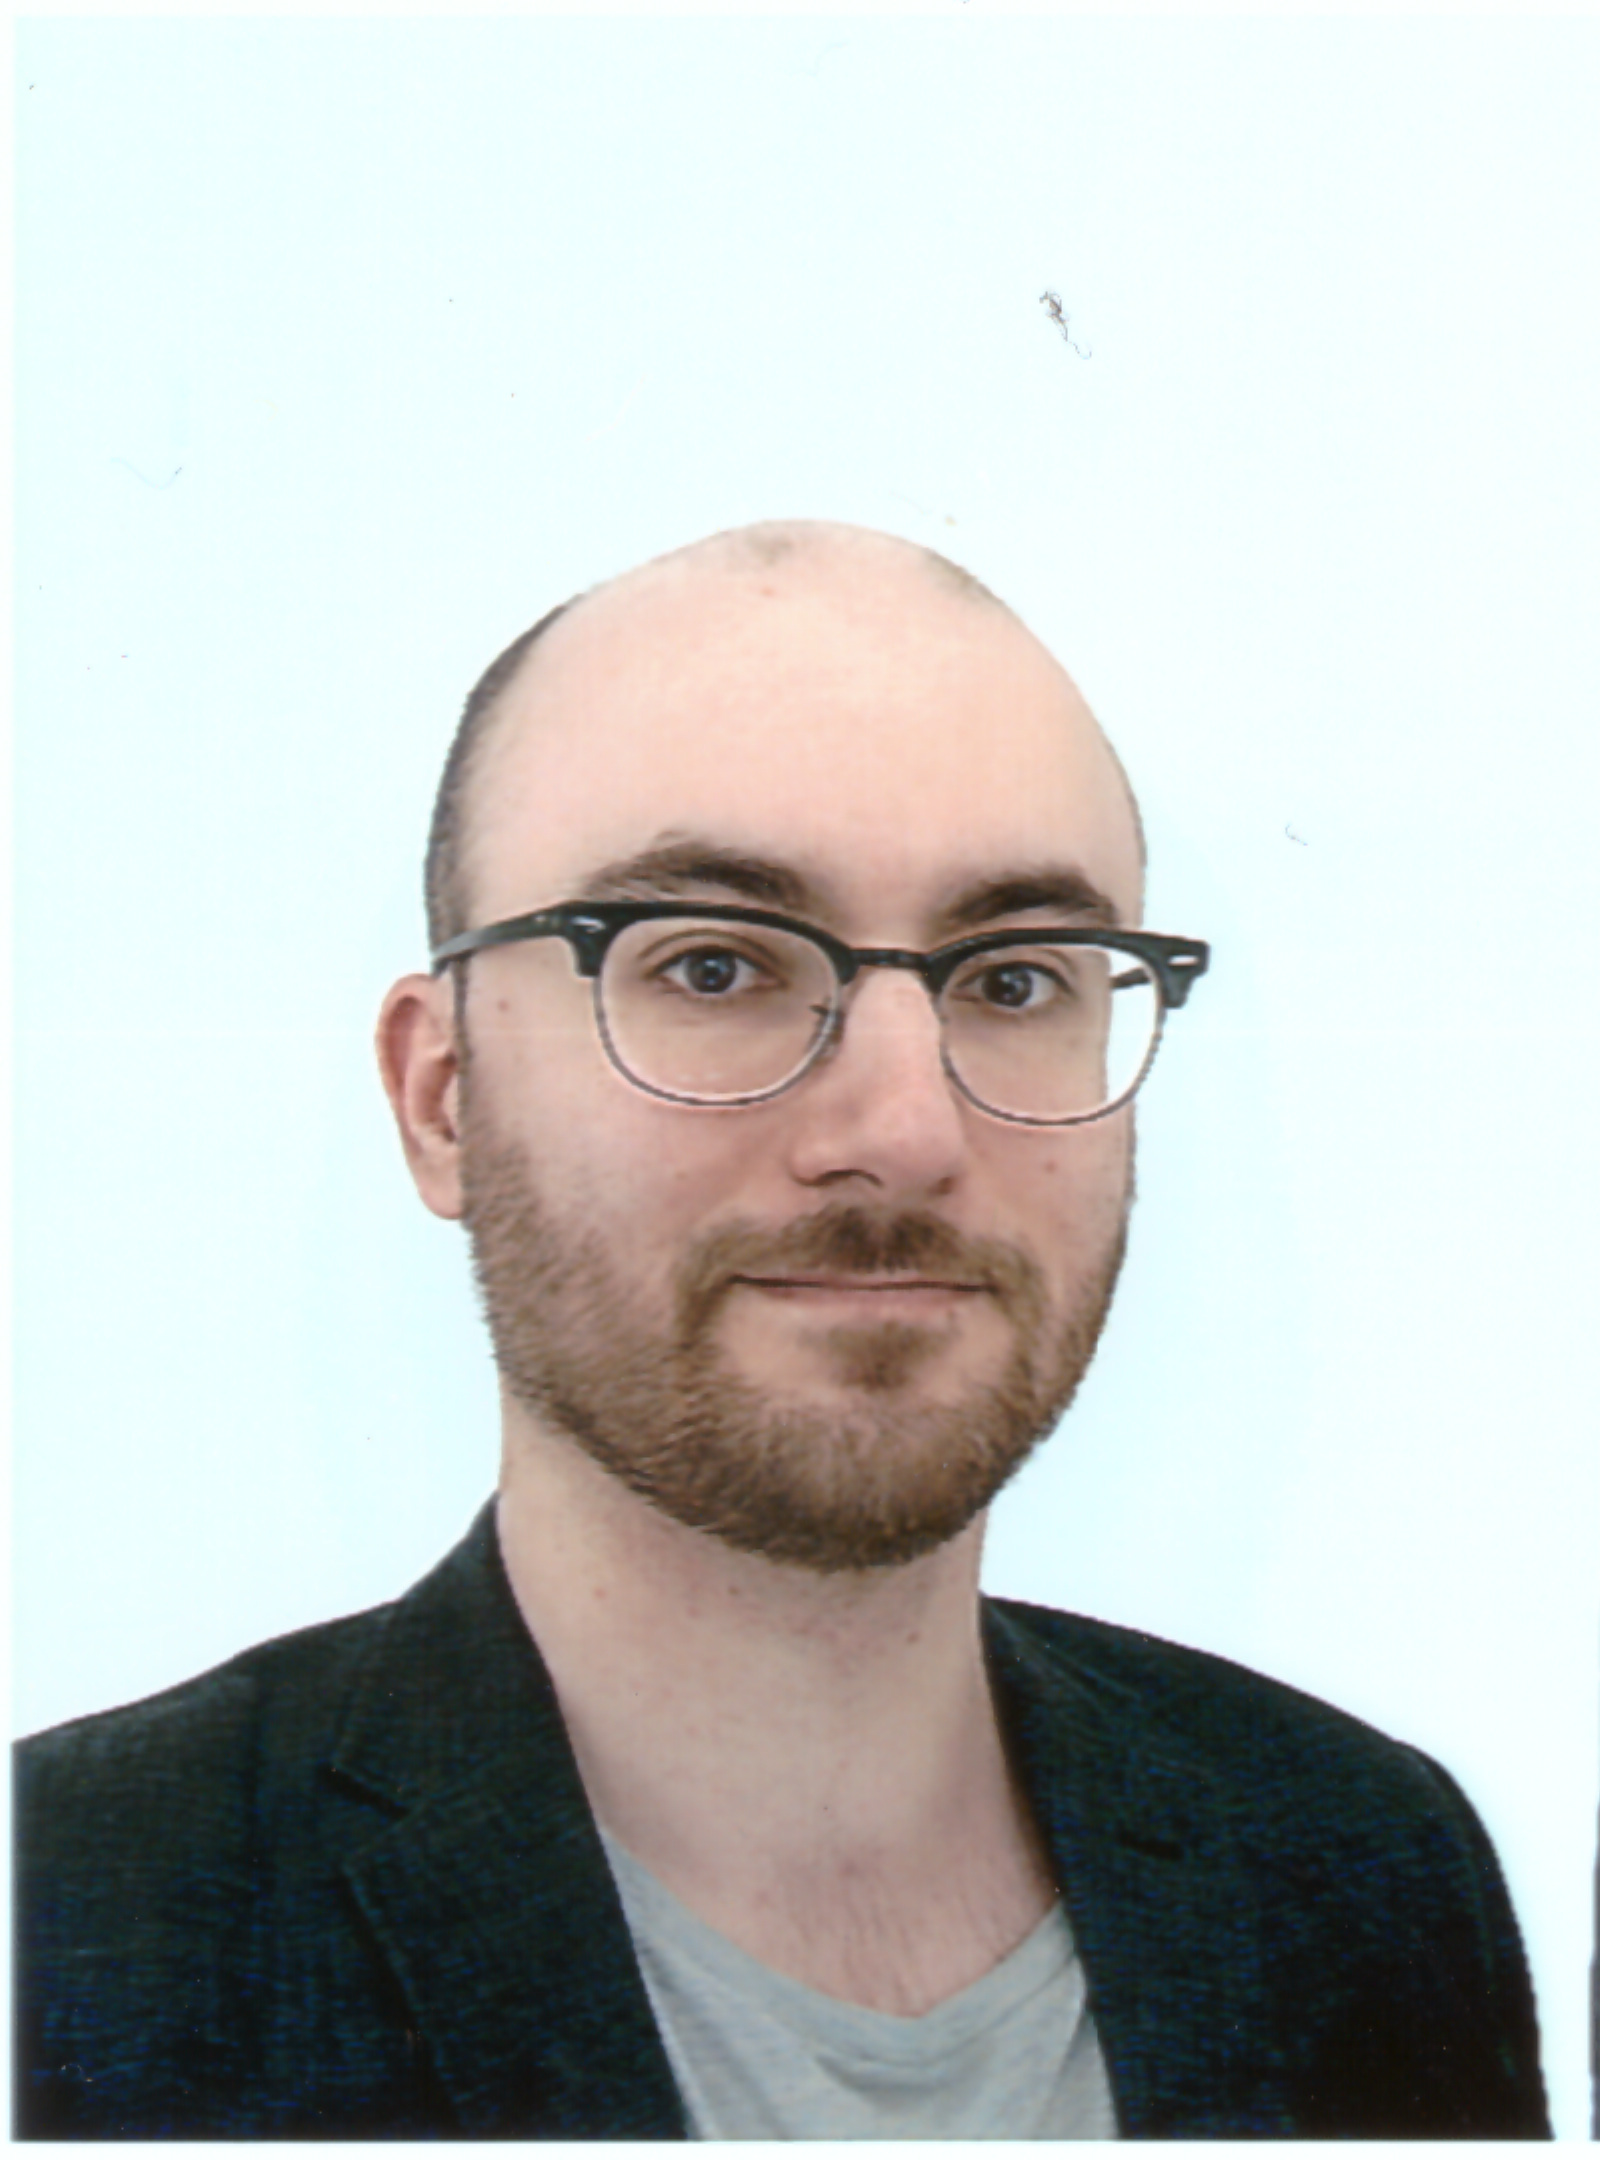
\includegraphics[trim=0cm 0cm 0cm 0.75cm, clip,scale = 0.92]{../../img/ichich2.png}};
%		\draw [anti-flashwhite, rounded corners=0\ClipSep, line width=0]
%		(current bounding box.north west) --
%		(current bounding box.north east) --
%		(current bounding box.south east) --
%		(current bounding box.south west) -- cycle
%		;
%	\end{tikzpicture}\\
	\faMapMarker~ Potsdam, Deutschland\\

	\vspace{0.15cm}
	{\color{pblue}\faPhone}	+49 174/6507598

	\vspace{0.15cm}
	{\color{pblue}\faEnvelope}~\href{mailto:silvio{\_}schwarz@web.de}{silvio{\_}schwarz@web.de}%\href{mailto:admin@silvioschwarz.com}{admin@silvioschwarz.com}\\

	\vspace{0.25cm}

	{\Large
		%\href{https://www.silvioschwarz.com}{\faHome} \hfill 
		\href{https://github.com/silvioschwarz}{\faGithub}  \hfill
		\href{silvioschwarz.}{\faSkype}
		\hfill \href{https://www.linkedin.com/in/silvioschwarz/}{\faLinkedin} \hfill
		\href{https://silvioschwarz.github.io}{\faGithubAlt} \hfill
		\href{ www.kaggle.com/amethodtomadness/}{
\includegraphics{../../img/kaggle.png}}}

	%	\section*{\hfill \fontsize{18pt}{24pt}\selectfont \color{pblue} Global Experience}
	%	\vspace{-2mm}
	%	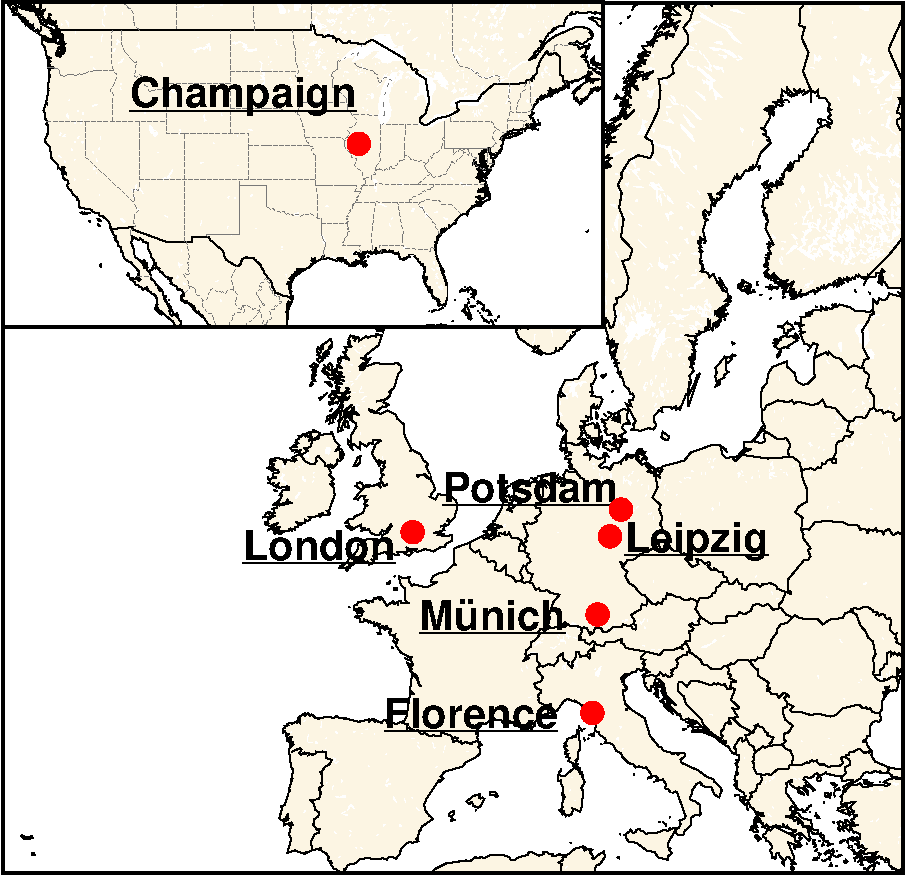
\includegraphics[trim=0cm 0cm 0cm 0cm, clip,scale=0.38]{../../img/globalEXPENG.pdf}
	\vspace{2mm}
	\hrule
	\vspace{-3mm}
	\section*{\fontsize{18pt}{24pt}\selectfont \color{pblue} Programmierung}
	\vspace{0.5mm}
	\textbf{\LARGE \faLinux}
\includegraphics[scale=0.50]{../../img/5stars.png}\\
	\textbf{\LARGE \faWindows}
\includegraphics[scale=0.50]{../../img/3stars.png}\\
	\vspace{5mm}

	\begin{tikzpicture}[node distance = 7mm, terminal/.style={
					rectangle, minimum height = 2mm, rounded corners = 1mm, thick,
					draw = darkgray, fill = white, align = left}]
		\node (A) [terminal] {Python};
		\node (AA) [terminal, right=2mm of A.east,anchor=west] {R};
		\node (AAA) [terminal, right=2mm of AA.east,anchor=west] {Matlab};
		\node (C) [terminal, below=of A.west,anchor=west] {Mathematica};
		\node (CC) [terminal, right=2mm of C.east,anchor=west] {Latex};
		\node (D) [terminal, below=of C.west,anchor=west] {HTML/CSS/JS};
		\node (DD) [terminal, right=2mm of D.east,anchor=west] {ArcGIS};
		\node (E) [terminal, below=of D.west,anchor=west] {BASH};
		\node (F) [terminal, right=2mm of E.east,anchor=west] {QGIS};
		\node (FF) [terminal, right=2mm of F.east,anchor=west] {Git/GitHub};
		\node (G) [terminal, below=of E.west,anchor=west] {GMT};
		\node (GG) [terminal, right=2mm of G.east,anchor=west] {Tensorflow};
		\node (GGG) [terminal, right=2mm of GG.east,anchor=west] {PyTorch};
	\end{tikzpicture}

	\vspace{3mm}
	%\includegraphics[scale=0.3]{../../../img/Programmierung.pdf}

	\hrule
	\vspace{-2mm}
	\section*{\fontsize{18pt}{24pt}\selectfont \color{pblue} Sprachen}
	\vspace{-2mm}
	\begin{itemize}
		\centering
		\item[\textbf{Deutsch}] 
\includegraphics[trim=0cm 0.2cm 0cm 0cm, clip,scale=0.50]{../../img/5stars.png}\vspace{-2mm}
		\item[\textbf{Englisch}]  
\includegraphics[trim=0cm 0.15cm 0cm 0cm, clip,scale=0.50]{../../img/4stars.png}\vspace{-2mm}
		\item[\textbf{Italienisch}] 
\includegraphics[trim=0cm 0.2cm 0cm 0cm, clip,scale=0.5]{../../img/3stars.png}\vspace{-2mm}
		\item[\textbf{Französisch}]  
\includegraphics[trim=0cm 0.2cm 0cm 0cm, clip,scale=0.50]{../../img/2stars.png}
	\end{itemize}
	\hrule
	\vspace{-2mm}
	\section*{\fontsize{18pt}{24pt}\selectfont \color{pblue} Expertise}
	\vspace{-0.2mm}
	\begin{tikzpicture}[node distance = 7mm, terminal/.style={
					rectangle, minimum height = 2mm, rounded corners = 1mm, thick,
					draw = darkgray, fill = white, align = left}]
		\node (A) [terminal] {seismische Gefährdungsanalyse};
		\node (AAA) [terminal,  below=of A.west,anchor=west] {machine learning};
		\node (AAB) [terminal,  right=2mm of AAA.east,anchor=west] {deep learning};
		\node (AAAA) [terminal,  below=of AAA.west,anchor=west] {Bayes'sche Methoden };
		\node (C) [terminal,  below=of AAAA.west,anchor=west] {Zeitreihenanalyse};
	\end{tikzpicture}
	\vspace{-2mm}
	\hrule
	\vspace{-2mm}
	\section*{\fontsize{18pt}{24pt}\selectfont \color{pblue} Zertifikate}
	\centering
	\vspace{-2mm}
	\textbf{\color{pblue}\underline{Tensorflow}}\\
	\href{https://www.coursera.org/account/accomplishments/specialization/certificate/WNXPGV8FR3AF}{\color{pblue}Developer},
	\href{https://www.coursera.org/account/accomplishments/specialization/certificate/R4LSQ7AK8M83}{\color{pblue}Data and Deployment},
	\href{https://www.coursera.org/account/accomplishments/specialization/certificate/5DDY3GKK3YTV}{\color{pblue}Advanced Techniques},
	\href{https://www.coursera.org/account/accomplishments/specialization/certificate/KA3YGBWN8RM2}{\color{pblue}Generative Adversarial Networks (GANs)}\\
	%	%	\href{}{Natural Language Processing (NPL)}\\
	%	%	\href{}{IBM Full Stack-Cloudentwickler}
	\vspace{2mm}
	\hrule
	\vspace{-2mm}
	\centering
	\section*{\fontsize{18pt}{24pt}\selectfont \color{pblue} Interessen}
	\vspace{-2mm}
	\vfill
	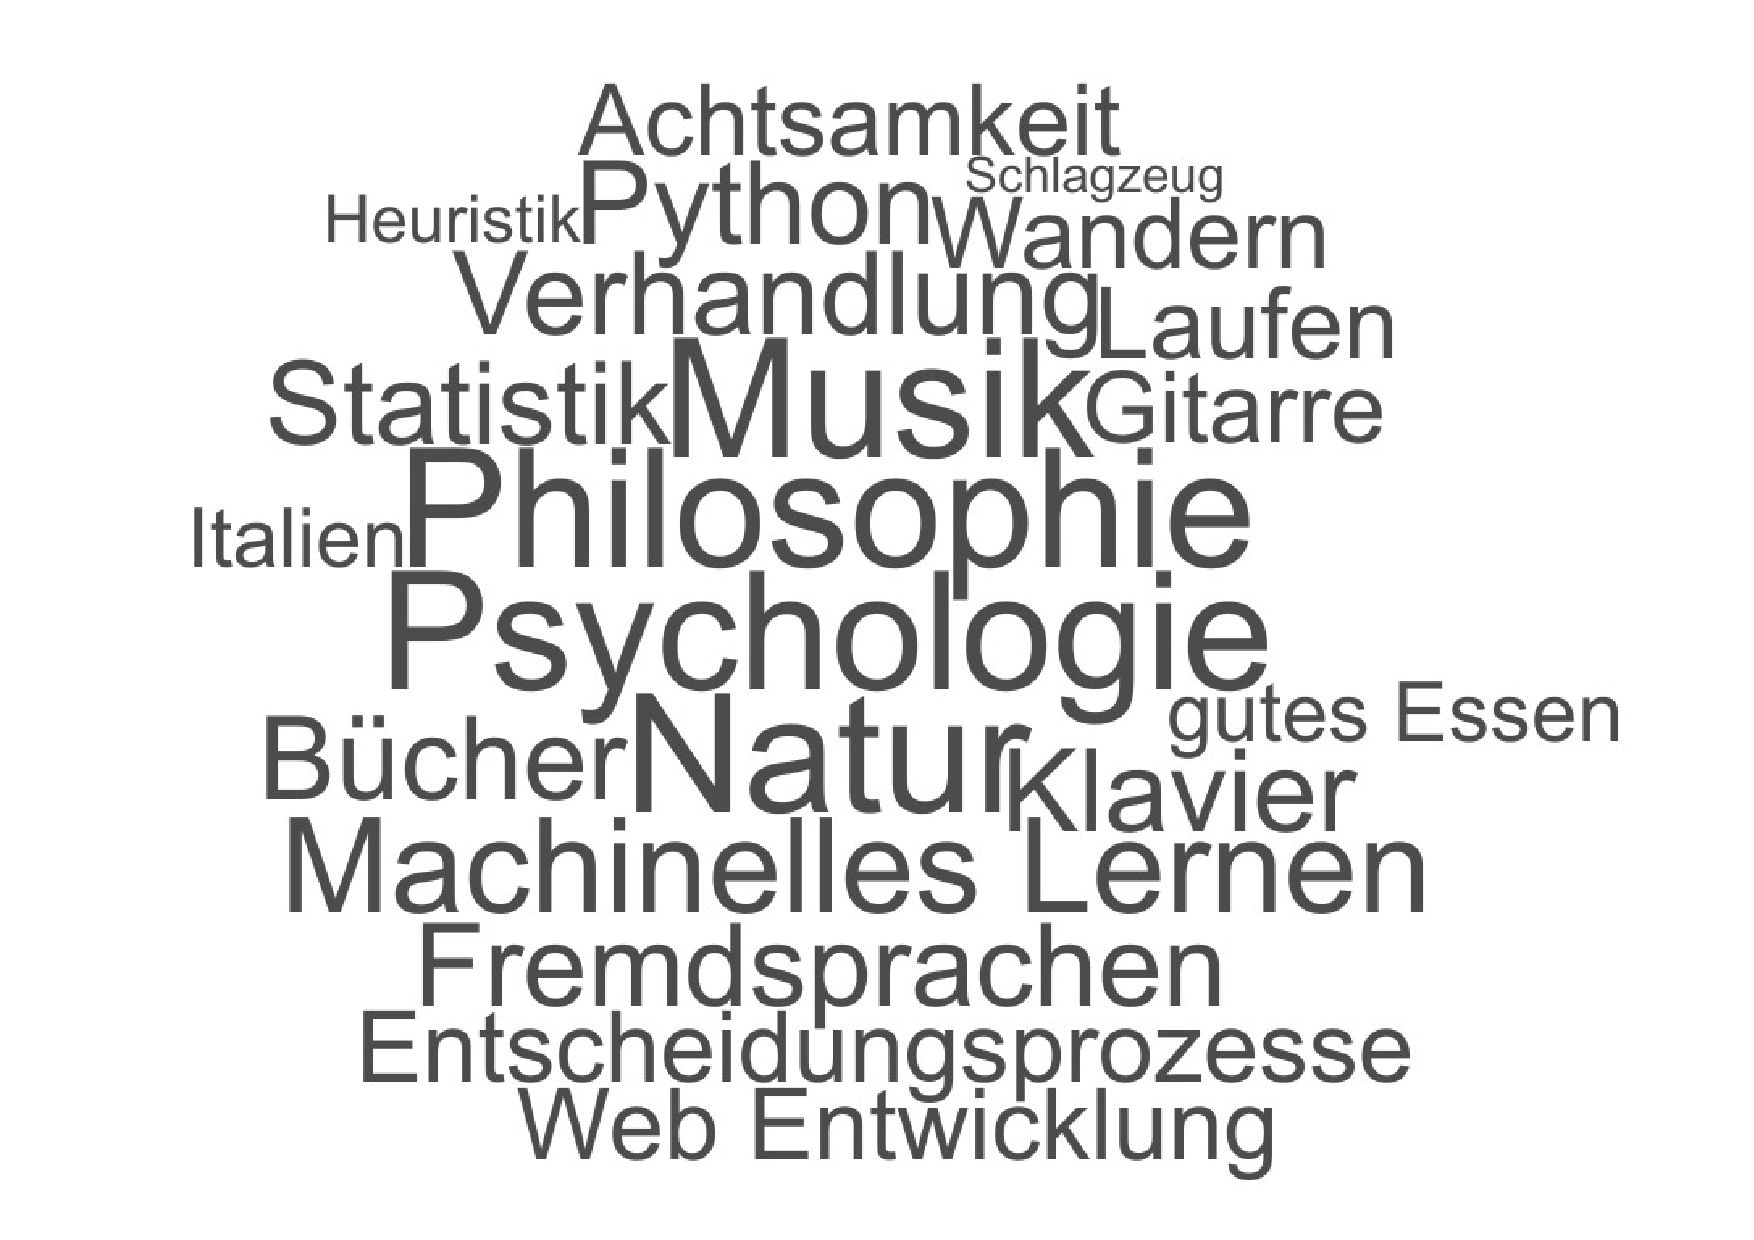
\includegraphics[trim=3cm 1cm 2cm 1cm, clip,scale=0.165]{../../img/wordcloudGER.pdf}

\end{minipage}
%%%%%%%%%%%%%%%%%%%%%%%%%%%%%%%%%%%%%%%%%%%%%%%%%%%%%%%%%%%%%%%%%%%%%%%%%%%%%%%%%%%%%%%%%%%%%%%%%%%
\hfill
\vrule
\hfill
\begin{minipage}[t]{0.70\textwidth}
	\vspace{0pt}
	%	\begin{minipage}[t]{0.49\textwidth}
	{\fontsize{30pt}{62pt}\color{gray} \selectfont {Silvio}{\textbf{Schwarz}}}\\
	{\fontsize{14pt}{24pt}\color{pblue} \selectfont Geophysiker \color{lightgray} (B.Sc.)}\\
	\hrule
	\section*{\fontsize{18pt}{24pt}\selectfont \color{pblue} Bildung}
	\begin{minipage}[t]{\minipageSmallEd\textwidth}
		\raggedleft
		2011 - 2019\\(8 Jahre)
	\end{minipage}
	\hfill
	\begin{minipage}[t]{\minipageBigEd\textwidth}
		\textbf{\color{pblue}\faHourglassHalf~Master of Science \hfill
			\href{https://www.uni-potsdam.de/}{\color{pblue}Universität Potsdam}}\\
		\textbf{\underline{Geowissenschaftens}}\hfill{krankheitsbedingt abgebrochen}\\
		\textbf{\underline{Vertiefung:}~Geophysik, machine learning}\\
		\textbf{\underline{Abschlussarbeit}}:\\ 1) \href{https://github.com/silvioschwarz/master-Abschlussarbeit}{Forecasting Macroseismic Intensities: A Sensitivity Study of a Bayesian Approach 2014-2016} \\
		2) Classification of eruptive tremor sources during the 2014-2015 Holuhraun sequence, Iceland 2019
	\end{minipage}\\\\\\
	\hfill
	\begin{minipage}[t]{\minipageSmallEd\textwidth}
		\raggedleft
		2008 - 2011\\(3 Jahre)
	\end{minipage}
	\hfill
	\begin{minipage}[t]{\minipageBigEd\textwidth}
		\textbf{\href{https://www.dropbox.com/s/297g1chiby8mrd3/Bachelor-Certificate.pdf?dl=0}{\color{pblue}\faGraduationCap~Bachelor of Science \hfill	\href{https://www.uni-potsdam.de/}{\color{pblue}Universität Potsdam}}}\\
		\textbf{\underline{Geowissenschaftens}}\\
		\textbf{Geologie, Mathematik, Physik, Chemie}\\
		\textbf{\underline{Abschlussarbeit}}:\\
		\href{https://www.dropbox.com/s/3kngo4hpb0c47ww/Bachelorarbeit.pdf?dl=0}{\pdftooltip{Simulation von Bodenbewegungsszenarien von Starkbeben (Deutsch)}{engl.: Simulating Bodenbewegungsmodellierung Scenarios of strong Earthquakes}} \\
	\end{minipage}
	\hfill
	\begin{minipage}[t]{\minipageSmallEd\textwidth}
		\raggedleft
		2000 - 2008\\(8 Jahre)
	\end{minipage}
	\hfill
	\begin{minipage}[t]{\minipageBigEd\textwidth}
		\textbf{\href{https://www.dropbox.com/s/nsgmvy7o64xb9si/Abiturzeugnis.pdf?dl=0}{\color{pblue}\faGraduationCap~Abitur \hfill \href{https://www.klosterschule.de/}{\color{pblue}Klosterschule Roßleben (staatl. Gymnasium)}}}\\
		\textbf{Mathematik}, \textbf{Geography}\\
		\textbf{\underline{Abschlussarbeit}}:\\
		\pdftooltip{Naturkatastrophen und ihr Einfluss auf das Leben in der Gegenwart (Deutsch)}{engl.: Natural Disasters and their Impact on Life in the Present}
	\end{minipage}\\\\
	\hrule
	%%%%%%%%%%%%%%%%%%%%%%%%%%%%%%%%%%%%%%%%%%%%%%%%%%%%%%%%%%%%%%%%%%%%%%%%%%%%%%%%%
	\section*{\fontsize{18pt}{24pt}\selectfont \color{pblue} Erfahrung}
	%	\begin{minipage}[t]{0.65\textwidth} 
	%		\begin{minipage}[t]{\minipageSmall\textwidth}
	%			\centering
	%			11/2017 - 03/2018\\(5 Monate)
	%		\end{minipage}
	%		\hfill
	%		\begin{minipage}[t]{\minipageBig\textwidth}
	%			\textbf{Werksstudent}\hfill \href{https://assecor.de/}{\color{pblue}DB Dialog}\\
	%			support passenger rights
	%		\end{minipage}
	%
	%		\vspace{\spacingWork}
	%

	\begin{minipage}[t]{\minipageSmall\textwidth}
		\raggedleft
		2019 \\(6 Monate)
	\end{minipage}
	\hfill
	\begin{minipage}[t]{\minipageBig\textwidth}
		\textbf{studentische Hilfskraft\hfill
		\href{https://www.geo.uni-potsdam.de/}{\color{pblue}Universität Potsdam}}\\
		\href{http://www.geo.uni-potsdam.de/allgemeine-geophysik-1570.html}{Arbeitsgruppe Allgemeine Geophysik}\\
		Charakterisierung von Tremorquellen während der Holuhraun Eruption, Island\\
		\textbf{\underline{Betreuung}}: \href{mailto:eva.eibl@un-potsdam.de }{\color{pblue}Prof. Dr. Eva Eibl }
	\end{minipage}

	%		\vspace{\spacingWork}
	%		
	%				\begin{minipage}[t]{0.25\textwidth}
	%				\centering
	%				01/2013\\ -\\ 04/2013 \\(3 Monate)
	%				\end{minipage}
	%				\hfill
	%				\begin{minipage}[t]{\minipageBig\textwidth}
	%				\textbf{Praktikum}\footnote{cancelled due to illness}\hfill	
	%				\href{https:///www.munichre.com/}{\color{pblue}Munich Re}\\
	%				Improvement of GMPE\\
	%				\textbf{\underline{Betreuung}}: \href{mailto:MKaeser@munichre.com}{\color{pblue}Prof. Dr. Martin Käser}%https://www.geophysik.uni-muenchen.de/Members/kaeser/cv
	%				\end{minipage}

	\vspace{\spacingWork}

	\begin{minipage}[t]{\minipageSmall\textwidth}
		\raggedleft
		2014 - 2015\\(11 Monate)
	\end{minipage}
	\hfill
	\begin{minipage}[t]{\minipageBig\textwidth}
		\textbf{Werksstudent\hfill
		\href{https://assecor.de/}{\color{pblue}Assecor GmbH, Berlin}}\\
		Dokumentation des Berliner Stromnetzes in einem Netzinformationssystem für Vattenfall Europe Sales GmbH
	\end{minipage}

	\vspace{\spacingWork}

	\begin{minipage}[t]{\minipageSmall\textwidth}
		\raggedleft
		2013 - 2014 \\(5 Monate)
	\end{minipage}
	\hfill
	\begin{minipage}[t]{\minipageBig\textwidth}
		\textbf{Werksstudent\hfill \href{https://assecor.de/}{\color{pblue}Assecor GmbH, Berlin}}\\
		Migration der IT Infrastruktur für BIOTRONIK SE \& Co. KG
	\end{minipage}

	\vspace{\spacingWork}

	\begin{minipage}[t]{\minipageSmall\textwidth}
		\raggedleft
		2012 \\(3 Monate)
	\end{minipage}
	\hfill
	\begin{minipage}[t]{\minipageBig\textwidth}
		\textbf{Master Praktikum\hfill
		\href{https:///www.wolframalpha.com/}{\color{pblue}Wolfram$\mid$Alpha, Illinois, USA}}\\
		Entwicklung von geophysikalischen Inhalt für Wolfram$~\mid~$Alpha\hfill \href{https://m.wolframalpha.com/input/?i=moment+magnitude}{\color{pblue}Example}\\
		\textbf{\underline{Betreuung}}: \href{mailto:bjornz@wolfram.com }{\color{pblue}Dr. Björn Zimmermann} \&	\href{mailto:mtrott@wolfram.com }{\color{pblue} Dr. Michael Trott}
	\end{minipage}

	\vspace{\spacingWork}

	\begin{minipage}[t]{\minipageSmall\textwidth}
		\raggedleft
		2011 - 2012\\(1 Jahr\\ 3 Monate)
	\end{minipage}
	\hfill
	\begin{minipage}[t]{\minipageBig\textwidth}
		\textbf{studentische Hilfskraft\hfill
		\href{https://www.uni-potsdam.de/}{\color{pblue}Universität Potsdam}}\\
		SSHAC LEVEL 3 PSHA Modellerstellung und Beratung\\
		1-wöchige Beratung für \href{https://www.imperial.ac.uk/people/j.bommer}{\color{pblue}Prof. Julian J. Bommer}, Imperial College London\\
		\textbf{\underline{Betreuung}:} \href{http://www.geo.uni-potsdam.de/mitarbeiterdetails/show/96/Frank_Scherbaum.html/}{\color{pblue}Prof. Frank Scherbaum}
	\end{minipage}

	\vspace{\spacingWork}

	\begin{minipage}[t]{\minipageSmall\textwidth}
		\raggedleft
		03/2011\\(1 Monat)
	\end{minipage}
	\hfill
	\begin{minipage}[t]{\minipageBig\textwidth}
		\textbf{Bachelor Praktikum\hfill
		\href{http://geologie.physgeo.uni-leipzig.de}{\color{pblue}Universität Leipzig}}\\
		Wartung des seismologischen Netzwerkes von Sachsen\\
		\textbf{\underline{Betreuung}}: \href{mailto:sfunke@rz.uni-leipzig.de}{\color{pblue}Dipl. Geophys. S. Funke}
	\end{minipage}\\\\
%	\hrule
		%%%%%%%%%%%%%%%%%%%%%%%%%%%%%%%%%%%%%%%%%%%%%%%%%%%%%%%%%%%%%%%%%%%%%%%%%%%%%%%%%
%		\section*{\fontsize{18pt}{24pt}\selectfont \color{pblue} Projekte}
%		\textbf{\color{pblue}\href{https://earthquake-distances.herokuapp.com}{EQDist}}\\ {Berechnung und Visualisierung von Distanzen für Bodenbewegungsmodellierung} \vspace{1mm} \\
%		\textbf{\color{pblue}\href{https://silvioschwarz.github.io/TerremotoPi/}{TerremotoPi}}\\ {Eine seismische Station auf Grundlage eines RaspberryPi mit Echtzeit Fähigkeiten!} \vspace{1mm}\\
%		\textbf{\color{pblue}\href{https://terrorxafrica.herokuapp.com}{TerrorXAfrica}}\\ {IBM cross-border effects challenge von bewaffneten Konfliketen im Rahmen des \href{https://hackhpi2019.devpost.com}{\color{pblue}HackHPI2019} }


\end{minipage}
\end{document}